\section{Phénoménologie des événements \Gjets}\label{chapter-JERC-section-pheno-GJets}
Les événements \Gjets\ peuvent être utilisés afin d'obtenir la correction résiduelle absolue en \pT\ des jets, introduite dans la section~\ref{chapter-JERC-section-CMS-subsec-residuals_pT}, ainsi que la résolution en énergie des jets. Les analyses correspondantes sont abordées dans les sections~\ref{chapter-JERC-section-JES} et~\ref{chapter-JERC-section-JER}.
\subsection{Principe des événements \Gjets\ et réponse balancée}
L'état final d'un événement \Gjets\ comporte un jet à calibrer d'une part et un photon utilisé comme objet de référence d'autre part.
En effet, les performances de reconstruction des photons sont meilleures que celles des jets. Sur la figure~\ref{fig-chapter-JERC-section-pheno-GJets-photon_resolution}, la résolution sur les photons est inférieure à \SI{4}{\%} et de l'ordre du pourcent dans le barillet. Dans le cas des jets, sur la figure~\ref{subfig-chapter-JERC-section-CMS-subsec-JER-JERC_RunI-Figure_036-b}, la résolution minimale est de \SI{5}{\%}.
L'utilisation de photons comme objet de référence est donc justifiée.
\begin{figure}[h]
\centering
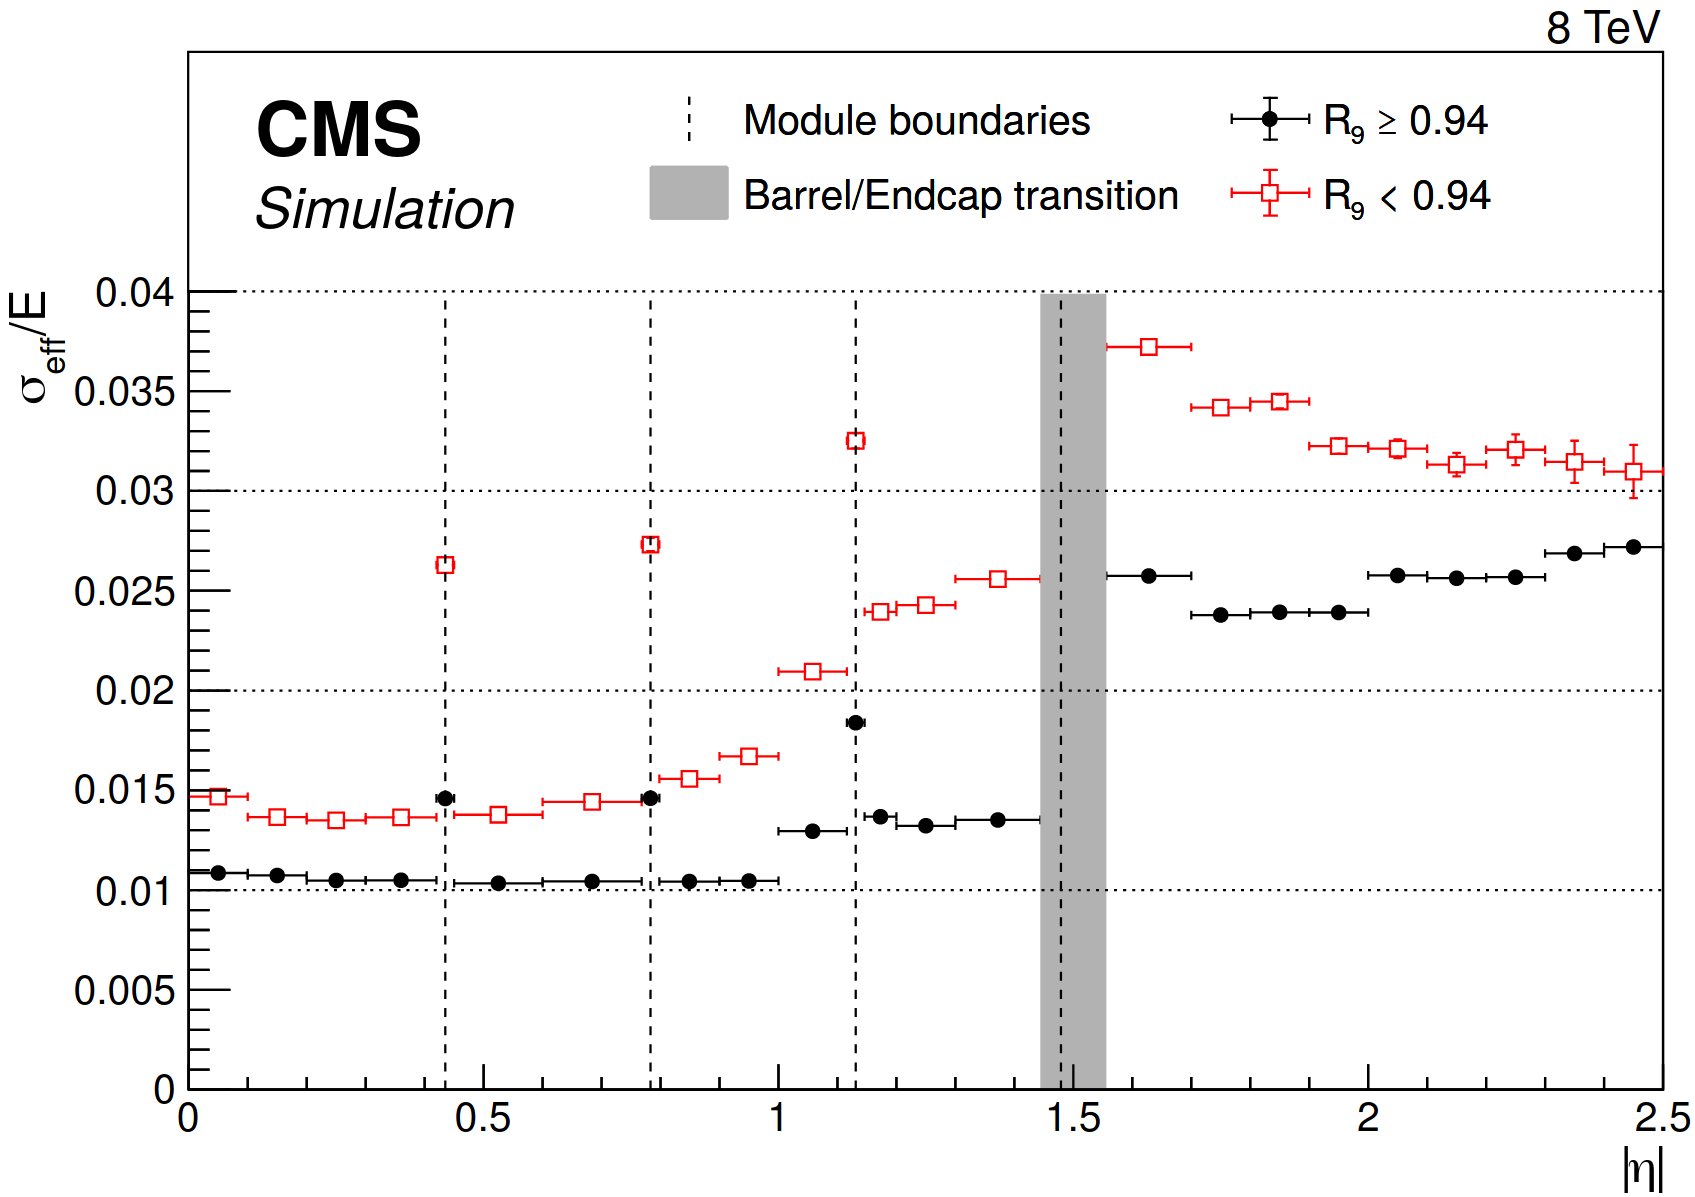
\includegraphics[width=.6\textwidth]{\PhDthesisdir/contents/chapter-JERC/phenomenologie/img_from_photon_ID_2015/photon_resolution.png}
\caption[Résolution en énergie des photons.]{Résolution relative en énergie des photons en fonction de $\eta$ pour des événements simulés $\higgs\to\photon\photon$~\cite{photon_ID_2015}. La variable $R_9$ est définie page~\pageref{eq-R9_definition}.}
\label{fig-chapter-JERC-section-pheno-GJets-photon_resolution}
\end{figure}
\par Des diagrammes de Feynman correspondant à des événements \Gjets\ sont présentés sur la figure~\ref{fig-fgraph-gamma_plus_jets}.
Ces événements ne comportent pas de neutrino issu de l'interaction dure\footnote{Des neutrinos peuvent apparaître lors de la formation du jet.}, il n'y a donc pas d'énergie transverse manquante due à la physique de ces événements.
L'impulsion transverse étant nulle dans l'état initial, par conservation, elle est nulle dans l'état final. Le photon et le jet sont donc balancés, \ie
\begin{equation}
\vpT_\ptcl^{\photon} + \vpT_\ptcl^\text{jet} = \vec{0}
\Rightarrow
\pT_\ptcl^{\photon} = \pT_\ptcl^\text{jet}
\mend
\end{equation}
\begin{figure}[h]
\centering\vspace{\baselineskip}
\subcaptionbox{\label{subfig-fgraph-gq_qGamma_S}}[.3\textwidth]
{\begin{fmffile}{gq_qGamma_S}\fmfstraight
\begin{fmfchar*}(20,20)
  \fmfleft{i1,i2}
  \fmfright{o1,o2}
  \fmf{gluon}{i2,v1}
  \fmf{fermion}{i1,v1,v2,o2}
  \fmf{photon}{v2,o1}
  \fmflabel{\gluon}{i2}
  \fmflabel{\quark}{i1}
  \fmflabel{\quark}{o2}
  \fmflabel{\photon}{o1}
  \fmfdot{v1,v2}
\end{fmfchar*}
\end{fmffile}\vspace{\baselineskip}}
\hfill
\subcaptionbox{\label{subfig-fgraph-gq_qGamma_T}}[.3\textwidth]
{\begin{fmffile}{gq_qGamma_T}\fmfstraight
\begin{fmfchar*}(20,20)
  \fmfleft{i1,i2}
  \fmfright{o1,o2}
  \fmf{gluon}{i2,v2}
  \fmf{fermion}{i1,v1,v2,o2}
  \fmf{photon}{v1,o1}
  \fmflabel{\gluon}{i2}
  \fmflabel{\quark}{i1}
  \fmflabel{\quark}{o2}
  \fmflabel{\photon}{o1}
  \fmfdot{v1,v2}
\end{fmfchar*}
\end{fmffile}\vspace{\baselineskip}}
\hfill
\subcaptionbox{\label{subfig-fgraph-qq_gGamma}}[.3\textwidth]
{\begin{fmffile}{qq_gGamma}\fmfstraight
\begin{fmfchar*}(20,20)
  \fmfleft{i1,i2}
  \fmfright{o1,o2}
  \fmf{gluon}{v2,o2}
  \fmf{fermion}{i1,v1,v2,i2}
  \fmf{photon}{v1,o1}
  \fmflabel{\antiquark}{i2}
  \fmflabel{\quark}{i1}
  \fmflabel{\gluon}{o2}
  \fmflabel{\photon}{o1}
  \fmfdot{v1,v2}
\end{fmfchar*}
\end{fmffile}\vspace{\baselineskip}}
\caption[Diagrammes de Feynman donnant un photon et un jet dans l'état final.]{Exemples de diagrammes de Feynman de processus physiques donnant un photon et un jet dans l'état final.}
\label{fig-fgraph-gamma_plus_jets}
\end{figure}
\par L'impulsion transverse du jet doit donc être égale à celle du photon, objet de référence.
La bonne résolution en énergie sur les photons permet de considérer que leur impulsion transverse au niveau reconstruit est égale à leur impulsion transverse au niveau particule.
Ainsi, la méthode de la balance\footnote{La méthode de la balance est introduite dans la section~\ref{chapter-JERC-section-CMS-subsec-residuals}.} permet de définir
\begin{equation}
\Rbal = \frac{\pT_\reco^\text{jet}}{\pT^{\photon}}
\mend[,]
\end{equation}
qui doit valoir 1 après correction.
Cette méthode est performante pour les événements à un photon et un jet dont la topologie est représentée sur la figure~\ref{subfig-Gamma_plus_jet_basic_event}.
\begin{figure}[h]
\centering
\subcaptionbox{Topologie typique des événements correspondant aux diagrammes de la figure~\ref{fig-fgraph-gamma_plus_jets}.\label{subfig-Gamma_plus_jet_basic_event}}[.45\textwidth]
{\includegraphics[width=.45\textwidth,height=.25\textheight,keepaspectratio]{\PhDthesisdir/plots_and_images/Event_displays/JERC/Gamma_plus_jet.tex}}
\hfill
\subcaptionbox{Topologie typique des événements correspondant au diagramme de la figure~\ref{subfig-fgraph-gq_qGamma_S-FSR_2jets}.\label{subfig-Gamma_plus_two_jets}}[.45\textwidth]
{\includegraphics[width=.45\textwidth,height=.25\textheight,keepaspectratio]{\PhDthesisdir/plots_and_images/Event_displays/JERC/Gamma_plus_2jets.tex}}
\caption{Topologies typiques des événements \Gjets.}
\label{fig-Gamma_plus_jet_events}
\end{figure}
\subsection{Effets radiatifs et activité additionnelle}\label{chapter-JERC-section-pheno-GJets-subsec-alpha_definition}
Des effets radiatifs peuvent survenir et altérer la topologie des événements \Gjets.
Un photon peut ainsi être radié dans l'état initial (ISR, \emph{Initial State Radiation}) ou dans l'état final (FSR, \emph{Final State Radiation}), ce qui correspond aux diagrammes de Feynman des figures~\ref{subfig-fgraph-gq_qGamma_S-ISR_2photons} et~\ref{subfig-fgraph-gq_qGamma_S-FSR_2photons}.
Un système composé d'un des photons et du jet n'est donc pas balancé dans ce cas.
Il est possible de supprimer ce biais en imposant la présence d'un seul photon dans l'événement.
La section efficace de production d'événements \Gjets\ à \SI{13}{\TeV} est importante~\cite{Gjet_xsec_2018}, il est donc possible de sélectionner de manière stricte les événements afin d'obtenir une bonne pureté tout en conservant une statistique suffisante.
\begin{figure}[h]
\centering\vspace{\baselineskip}
\subcaptionbox{\label{subfig-fgraph-gq_qGamma_S-ISR_2jets}}[.225\textwidth]
{\begin{fmffile}{gq_qGamma_S-ISR_2jets}\fmfstraight
\begin{fmfchar*}(20,20)
  \fmfleft{i1,i2}
  \fmfright{o0,o1,o2}
  \fmf{gluon}{i2,v1}
  \fmf{phantom}{i1,v1}
  \fmf{phantom, tension=2}{v1,v2}
  \fmf{phantom}{v2,o2}
  \fmf{phantom}{v2,o0}
  \fmflabel{\gluon}{i2}
  \fmflabel{\quark}{i1}
  \fmflabel{\quark}{o2}
  \fmflabel{\photon}{o1}
  \fmfdot{v1,v2}
  \fmffreeze
  \fmf{fermion}{i1,v3,v1,v2,o2}
  \fmffreeze
  \fmf{photon}{v2,o1}
  \fmf{gluon}{v3,o0}
  \fmflabel{\gluon}{o0}
  \fmfdot{v3}
\end{fmfchar*}
\end{fmffile}\vspace{\baselineskip}}
\hfill
\subcaptionbox{\label{subfig-fgraph-gq_qGamma_S-ISR_2photons}}[.225\textwidth]
{\begin{fmffile}{gq_qGamma_S-ISR_2photons}\fmfstraight
\begin{fmfchar*}(20,20)
  \fmfleft{i1,i2}
  \fmfright{o0,o1,o2}
  \fmf{gluon}{i2,v1}
  \fmf{phantom}{i1,v1}
  \fmf{phantom, tension=2}{v1,v2}
  \fmf{phantom}{v2,o2}
  \fmf{phantom}{v2,o0}
  \fmflabel{\gluon}{i2}
  \fmflabel{\quark}{i1}
  \fmflabel{\quark}{o2}
  \fmflabel{\photon}{o1}
  \fmfdot{v1,v2}
  \fmffreeze
  \fmf{fermion}{i1,v3,v1,v2,o2}
  \fmffreeze
  \fmf{photon}{v2,o1}
  \fmf{photon}{v3,o0}
  \fmflabel{\photon}{o0}
  \fmfdot{v3}
\end{fmfchar*}
\end{fmffile}\vspace{\baselineskip}}
\hfill
\subcaptionbox{\label{subfig-fgraph-gq_qGamma_S-FSR_2jets}}[.225\textwidth]
{\begin{fmffile}{gq_qGamma_S-FSR_2jets}\fmfstraight
\begin{fmfchar*}(20,20)
  \fmfleft{i1,i2}
  \fmfright{o1,o0,o2}
  \fmf{gluon}{i2,v1}
  \fmf{phantom}{i1,v1}
  \fmf{phantom, tension=2}{v1,v2}
  \fmf{phantom}{v2,o2}
  \fmf{photon}{v2,o1}
  \fmflabel{\gluon}{i2}
  \fmflabel{\quark}{i1}
  \fmflabel{\quark}{o2}
  \fmflabel{\photon}{o1}
  \fmfdot{v1,v2}
  \fmffreeze
  \fmf{fermion}{i1,v1,v2,v3,o2}
  \fmffreeze
  \fmf{gluon}{v3,o0}
  \fmflabel{\gluon}{o0}
  \fmfdot{v3}
\end{fmfchar*}
\end{fmffile}\vspace{\baselineskip}}
\hfill
\subcaptionbox{\label{subfig-fgraph-gq_qGamma_S-FSR_2photons}}[.225\textwidth]
{\begin{fmffile}{gq_qGamma_S-FSR_2photons}\fmfstraight
\begin{fmfchar*}(20,20)
  \fmfleft{i1,i2}
  \fmfright{o1,o0,o2}
  \fmf{gluon}{i2,v1}
  \fmf{phantom}{i1,v1,v2,o2}
  \fmf{photon}{v2,o1}
  \fmflabel{\gluon}{i2}
  \fmflabel{\quark}{i1}
  \fmflabel{\quark}{o2}
  \fmflabel{\photon}{o1}
  \fmfdot{v1,v2}
  \fmffreeze
  \fmf{fermion}{i1,v1,v2,v3,o2}
  \fmffreeze
  \fmf{photon}{v3,o0}
  \fmflabel{\photon}{o0}
  \fmfdot{v3}
\end{fmfchar*}
\end{fmffile}\vspace{\baselineskip}}
\caption[Diagrammes de Feynman de processus avec ISR ou FSR.]{Exemples de diagrammes de Feynman de processus avec ISR (\ref{subfig-fgraph-gq_qGamma_S-ISR_2jets}, \ref{subfig-fgraph-gq_qGamma_S-ISR_2photons}) ou FSR (\ref{subfig-fgraph-gq_qGamma_S-FSR_2jets}, \ref{subfig-fgraph-gq_qGamma_S-FSR_2photons}) donnant des événements avec deux jets (\ref{subfig-fgraph-gq_qGamma_S-ISR_2jets}, \ref{subfig-fgraph-gq_qGamma_S-FSR_2jets}) ou deux photons (\ref{subfig-fgraph-gq_qGamma_S-ISR_2photons}, \ref{subfig-fgraph-gq_qGamma_S-FSR_2photons}) dans l'état final.}
\label{fig-fgraph-gamma_plus_jets-ISR-FSR}
\end{figure}
\par L'ISR et le FSR peuvent aussi produire un gluon, ce qui correspond aux diagrammes de Feynman des figures~\ref{subfig-fgraph-gq_qGamma_S-ISR_2jets} et~\ref{subfig-fgraph-gq_qGamma_S-FSR_2jets}.
Plusieurs jets sont alors présents dans l'état final et sont ordonnés par impulsion transverse décroissante.
Le cas de la figure~\ref{subfig-fgraph-gq_qGamma_S-ISR_2jets}, correspondant à un jet additionnel par ISR, peut être supprimé par une condition sur les directions du photon et du premier jet qui doivent être opposées.
Dans le cas du diagramme de la figure~\ref{subfig-fgraph-gq_qGamma_S-FSR_2jets}, correspondant à un jet additionnel par FSR, le photon est balancé avec le système des deux jets. La topologie d'un tel événement est illustrée sur la figure~\ref{subfig-Gamma_plus_two_jets}.
La réponse balancée est alors considérée entre le photon et le premier jet, \ie\ le jet d'impulsion transverse la plus grande. Ainsi,
\begin{equation}
\Rbal = \frac{\pT_\reco^\text{jet 1}}{\pT^{\photon}}
\mend
\end{equation}
\par La présence d'un jet secondaire, comme sur la figure~\ref{subfig-Gamma_plus_two_jets}, créé un déséquilibre dans \Rbal\ dû à la physique de l'événement et non à la JES. Il ne faut donc pas corriger cet effet.
Pour cela, il faut pouvoir se ramener au cas où un seul jet est présent, comme dans l'événement de la figure~\ref{subfig-Gamma_plus_jet_basic_event}.
L'activité additionnelle liée aux jets supplémentaires est quantifiée par la variable
\begin{equation}
\alpha = \frac{\pT_\reco^\text{jet 2}}{\pT^{\photon}}
\mend
\label{eq-chapter-JERC-definition_alpha}
\end{equation}
L'analyse des événements \Gjets\ est ainsi réalisée à différentes valeurs de $\alpha$, puis une extrapolation de \Rbal\ à $\alpha=0$ permet d'obtenir le résultat souhaité. Cette procédure est détaillée dans la section~\ref{chapter-JERC-section-JES}.
\subsection{Utilisation conjointe de la réponse MPF}
En complément de la réponse balancée, la réponse MPF, définie comme
\begin{equation}
\RMPF = 1 + \frac{\vpT^{\photon}\cdot\vMET}{\abs{\vpT^{\photon}}^2}
\mend[,]
\end{equation}
est également analysée.
Les impulsions de toutes les particules présentes étant considérées, \RMPF\ est moins sensible à l'activité additionnelle que \Rbal, ce qui se retrouve dans les résultats de l'analyse, figure~\ref{fig-chapter-JERC-section-JES-subsec-analyse-responsebal_and_MPF_eta0013_ptPhot_175_230_extrap}, page~\pageref{fig-chapter-JERC-section-JES-subsec-analyse-responsebal_and_MPF_eta0013_ptPhot_175_230_extrap}, où ces deux réponses sont représentées en fonction de $\alpha$.
\par L'utilisation de la réponse MPF nécessite une bonne reconstruction de \vMET, ce qui est le cas grâce aux bonnes performances de l'algorithme de \PF.
Son utilisation conjointe avec la réponse balancée permet d'obtenir des résultats complémentaires.
Des écarts significatifs observés entre les deux méthodes indiqueraient ainsi des effets incompris, nécessitant de plus amples investigations.
Dans la situation de la figure~\ref{fig-chapter-JERC-section-JES-subsec-analyse-responsebal_and_MPF_eta0013_ptPhot_175_230_extrap} par exemple, les rapports des réponses balancée et MPF entre données et simulations valent
$\num{0.967}\pm\num{0.001}$
et
$\num{0.966}\pm\num{0.001}$,
ce qui est tout à fait compatible.
